\begin{abstract}
Public videos attributed to extraterrestrial (ET) channeling offer a heterogeneous record of questions, advice, cosmological claims and platform presentation. Comparing this material requires distinguishing a practitioner from a publisher, a paraphrase from a spoken turn, and a generated response from source evidence. We connect a preserved \UploadN-upload index to \QAN\ question/answer-gist candidates from \QAVideoN\ Q\&A-bearing digests, all in one Darryl Anka-related practitioner context. We audit coverage, source dependence and possible reuse, compare question and answer vocabulary, and execute a grouped-source CPU retrieval and adaptation pilot. Across \MatchedN\ matched uploads, title/caption similarity rank association is \RawRankAssociation\ before and \ConditionedRankAssociation\ after measured length conditioning; this is a descriptive sensitivity. The local pilot separately exposes lexical reconstruction, unsupported responses and source-citation failures. New collection attempts, retained derivatives and executed model outputs remain distinct in the database, dashboard and reproducible artifacts. The contribution is an inspectable measurement resource for published discourse and computational source handling. Human construct validation, rights review, authorship and submission decisions remain pending; the study does not verify attributed communication origins or physical claims.
\end{abstract}

\section{Introduction}
Online audiences encounter extraordinary claims through a mixture of recordings, interviews, excerpts, summaries and search results. Each layer changes the question that a researcher can answer. A title reveals how an upload is presented; a caption records available recognized speech; a digest compresses that speech; and a language model generates a new response from a prompt and its accessible evidence. These layers can all be computationally compared, but their similarities refer to different objects.

Public ET-channeling videos make this problem concrete. Practitioners publicly attribute messages to named entities or collectives. Their material circulates through official accounts, interview shows, archives and repost publishers. Questions range from everyday relationships and life direction to contact, consciousness, history and physical mechanisms. A single recording may mix a host introduction, an audience question, a purported message and commercial promotion. One performance can reappear as several uploads, while one publisher can host many practitioners. Treating every account as a person or every upload as an independent session changes both denominators and interpretations.

The first Channeling Atlas release addressed the platform layer through source reconciliation, duration summaries, keyword indicators and title/caption representations. A subsequent expansion created an auditable question-answer candidate database. The present continuation integrates these layers and asks a more focused methodological question: how can a researcher move from a heterogeneous public-video index toward source-grounded question answering without losing the evidence type, source dependency or limits of the original material?

This question has two connected parts. The first concerns the corpus: whether question wording, answer wording, publisher structure, duration and source reuse explain apparent similarity. The second concerns computation: whether retrieval and limited adaptation can produce useful, source-addressable responses on held-out material, and what simple automated scores actually measure. Retrieval-augmented generation (RAG) can place evidence in a prompt, while parameter-efficient training can change a model's response behavior. Neither operation independently turns derivative summaries into validated propositions. A careful pilot must therefore preserve the distinction between reproducing a source account and determining whether that account is true.

We ask three research questions:
\begin{itemize}
\item \textbf{RQ1: Source structure.} What coverage, concentration, source dependence and possible reuse patterns constrain comparisons within the retained video and question-answer index?
\item \textbf{RQ2: Representation.} How do question and answer vocabulary, upload context and text-layer choices affect retrieval and similarity on matched, source-addressable units?
\item \textbf{RQ3: Local modeling.} What can a bounded CPU pilot establish about closed-book, retrieval-conditioned and parameter-efficient response generation when source/video dependencies are controlled and outputs are retained for inspection?
\end{itemize}

Our contribution is a linked measurement resource and executed exploratory investigation. It combines a frozen public-video index, typed derivative Q\&A records, transparent keyword extraction, source-family sensitivity, matched numerical diagnostics and a small local-model evaluation with an auditable result ledger. The manuscript and dashboard draw from the same result artifacts, while earlier releases remain preserved. Established methods---TF--IDF, cosine similarity, retrieval, channel centroids and low-rank adaptation---are used as baselines rather than presented as algorithmic inventions. The substantive scope is public discourse and its computational representation.

\section{Background and Related Work}
\subsection{Channeling content and equivalent questions}
Studies of channeling differ in whether they examine elicited participant responses, naturalistic communications or AI-mediated archival answers. These designs are related but not interchangeable. \citet{anastasia2020qualitative} analyze elicited content from thirteen trance channels using qualitative methods. \citet{wahbeh2023answers} compare responses to ten scientist-supplied questions, with quantitative correspondence examined in seven US participants and qualitative work spanning fifteen participants across two countries. Such designs foreground equivalent prompts and context. A shared theme need not imply agreement on a proposition.

The related prospective semantic and qualitative studies by Wahbeh and Glick describe a three-channeler research program \citep{wahbeh2026semantic,wahbeh2026qualitative}. The retained source register records accessible abstracts and supplement artifacts separately from publisher full text. Their relevance is methodological: comparisons should separate prompts, participants and conditions rather than pool all utterances into a universal similarity score.

A newer archival comparison ingests two text collections, queries each through a common UFODex system using the same questions, and compares generated answers \citep{wahbeh2026records}. Its methods also describe speech-recognition and embedding components. The public supplement directs both corpus queries toward a positive, supportive framing of the subject. A shared generator and prompt stance are therefore plausible contributors to generated resemblance. The computational unit is an AI-mediated archival response, rather than an observed original answer. This is a close comparator for our local-model branch, but its scores cannot be pooled with our title, caption or digest scores. Generated correspondence, original-source agreement and external verification remain separate evaluation targets.

Ethnographic studies of channeling and mediumship emphasize learned practices, voice and audience interaction \citep{klinoron2014channel,tomlinson2019medium}. Our access to these sources is recorded at abstract depth. Small-community research can provide rich contextual interpretation when it includes participant accounts and reflexive methods \citep{claisse2023faith}; a small computational corpus does not automatically inherit that grounding. Our model-assisted readings are interpretations of retained summaries, not participant ethnography.

\subsection{YouTube sampling and religious communication}
YouNiverse documents the construction and coverage of a large English-language channel/video metadata resource \citep{ribeiro2021youniverse}. The principle that transfers is procedural: acquisition and inclusion define the observable population. Our curated source union does not inherit YouNiverse's scale, thresholds or sampling weights. Updating every known ID improves within-index coverage without establishing a complete channel history or a census of practitioners.

Tube2Vec represents YouTube channels using sampled video titles and descriptions and evaluates channel representations on human tasks \citep{boesinger2024tube2vec}. It is a close computational precedent for account-level text vectors. Its design shows that channel-centroid embeddings are established practice; the present contribution concerns evidence-layer comparability and source dependencies in a much smaller, selected domain corpus. The publication is a peer-reviewed ICWSM poster paper, a status distinguished from an unreviewed software README.

\citet{chen2026digital} separate narratives, visual presentation and audience engagement in a religious YouTube study. Their published methods describe keyword-based API collection, explicit filtering, pilot codebook development and human review of model labels. Their annotation and held-out human-coded components provide a useful contrast to the present unvalidated keyword indicators. We borrow the ordering of questions, acquisition and validation; their reported reliability does not transfer to our codebook or model-generated summaries.

Other platform studies analyze comment pathways or trace content sharing across publishing surfaces \citep{ota2025pathways,starbird2018ecosystem}. Their operationalizations show why a proxy must be named for what it observes. We do not infer viewer pathways from repeated vocabulary or original authorship from similar uploads, and we do not transfer those studies' political categories to indexed practitioners.

\subsection{Text analysis, retrieval and adaptation}
Automatic content analysis requires validation for its substantive use \citep{grimmer2013text}. Topic evaluation distinguishes interpretable labels, statistical coherence and replication reliability \citep{chang2009reading,doogan2021twaddle,hoyle2021incoherence,schroeder2025reliability}. Fluent topic descriptions can still be generic without human involvement \citep{li2025haystack}. We therefore name the extraction mechanism---dictionary presence, lexical retrieval or a model annotation---rather than calling every output a validated theme.

Sentence-BERT and MiniLM provide efficient representation baselines \citep{reimers2019sentencebert,wang2020minilm}. Broader multilingual benchmarks demonstrate that performance depends on task and language \citep{muennighoff2023mteb,enevoldsen2025mmteb}. A familiar encoder or larger language model does not remove source attribution, duplicated performance or prompt-equivalence problems. In-domain held-out judgments remain necessary for substantive agreement claims.

Retrieval-augmented generation separates a generator from an external evidence store \citep{lewis2020rag}; REALM studies retrieval-augmented language-model pretraining \citep{guu2020realm}. These are relevant foundations rather than interchangeable implementations. The present pilot uses a small local model and lexical retrieval over permitted derivative records, not the full architectures, data or training regimes of those papers. The intervention is access to source-addressable context under a controlled split.

\citet{ovadia2024finetuning} compare fine-tuning and retrieval for knowledge injection on their evaluated tasks. Their result motivates measuring both routes under stated conditions, not a universal ranking of RAG over every adaptation method. \citet{gekhman2024hallucinations} show why learning new factual associations during fine-tuning warrants separate analysis of unsupported outputs. Low-rank adaptation reduces the trainable parameter subset \citep{hu2022lora}; efficiency does not establish that learned responses are correct, faithful to source or robust to paraphrase.

RAG evaluation frameworks separate properties such as contextual relevance and answer faithfulness rather than assigning a single undifferentiated quality score \citep{es2024ragas,saadfalcon2024ares}. Their model-based evaluation components and calibration requirements cannot be inherited merely by computing token overlap. We retain raw outputs and retrieved IDs, name each local proxy explicitly, and leave source entailment and human usefulness to future held-out validation.

Evidence location within long contexts can materially affect model performance \citep{liu2024lostmiddle}. Source duplication can also distort training and evaluation \citep{lee2022dedup}. These findings motivate bounded context, documented truncation and source/video grouping in our pilot. Our lexical source-family graph is a conservative leakage guard, not proof that all source duplication or pretraining contamination has been removed.


The new source register distinguishes freshly retrieved/read full texts, retained prior reading records, model cards and software documentation. This is a targeted methodological review, not a systematic review or a priority claim. Software repositories establish implementation choices and licenses; empirical papers support the methodological comparisons to their inspected access depth.

\section{Data and Source Transformations}
\subsection{A preserved multi-layer index}
The continuation resides in \texttt{occult-kranti/channels-ET}, imported from the earlier Atlas project. The original Bashar Index and previous manuscript releases remain separately preserved. Our primary frozen analytical snapshot contains \UploadN\ unique upload identifiers, \DurationN\ positive durations, \DateN\ exact upload dates and \TitleN\ English-likely eligible titles. These counts describe a convenience sample. Publication dates can date reposts, and relative age strings are not converted into invented dates.

The union originally combined 482 atlas IDs and 457 valid unique archive IDs, with fourteen overlaps. Account directories contain aliases, unresolved routes and empty historical leads. The discovery layer includes practitioner, lineage and partial-name candidates, plus adjacent spiritual/contextual material. Inclusion documents public description and source discovery; it does not certify that every upload is a channeling performance.

\begin{table}[t]
\centering\small\setlength{\tabcolsep}{3pt}
\begin{tabular}{p{0.58\columnwidth}p{0.18\columnwidth}p{0.15\columnwidth}}
\toprule
Evidence layer & Available & Indexed \\ \midrule
Publishing account resolved & 886 & 925 \\
Positive upload duration & 881 & 925 \\
Exact upload date & 880 & 925 \\
English-likely eligible title & 742 & 925 \\
Frozen English caption pilot & 30 & 925 \\
\bottomrule
\end{tabular}
\caption{Frozen source coverage. The caption row denotes selected pilot inclusion, not estimated caption availability.}
\end{table}

The identity model distinguishes a practitioner, publishing account, upload, original session, text artifact and attributed entity label. These relations are many-to-many. Only explicit supported alias edges are merged. Unique upload IDs remove URL duplication, not repeated performances. The same practitioner can appear on several interview accounts; treating those publishers as different mediums would create artificial cross-person agreement.

\begin{figure*}[t]
\centering
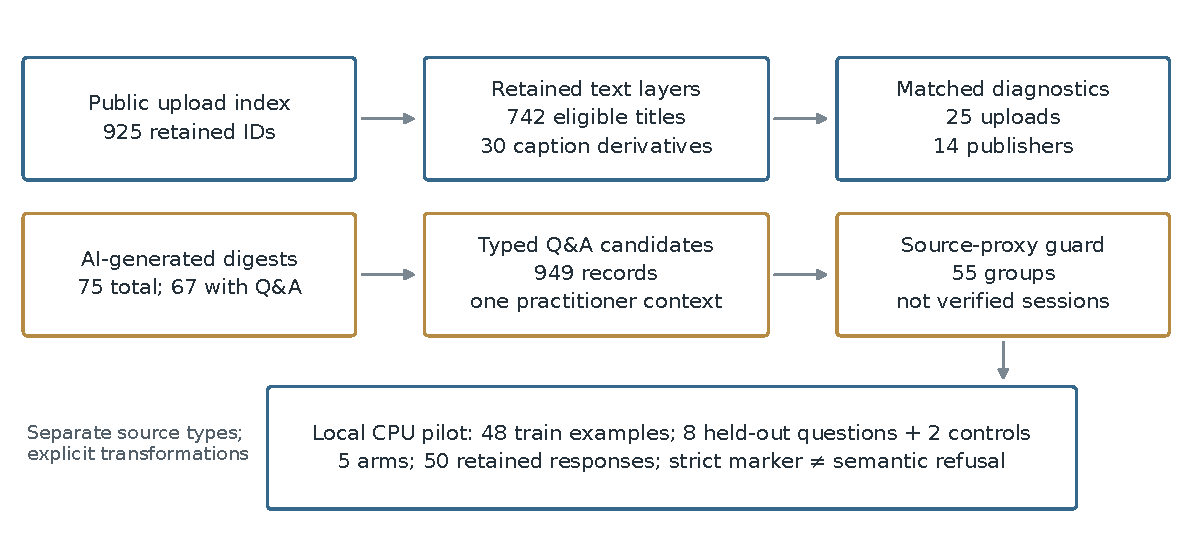
\includegraphics[width=\textwidth]{generated/figures/evidence-flow.pdf}
\caption{Evidence transformations in the executed resource. Public metadata, retained text derivatives, AI-digest candidates and model responses remain separate types. Source-proxy groups are conservative leakage guards rather than verified original performances. The original five-arm pilot is distinct from later diagnostic controls.}
\label{fig:evidenceflow}
\end{figure*}

\subsection{Captions, digests and Q\&A candidates}
The retained caption pilot attempted 36 uploads, retrieved 34 tracks and retained 30 English documents for balanced analysis. Most offered tracks were automatic; the platform's manual flag is not an accuracy audit. Hosts and promotion remain unsegmented. Numeric derivatives are retained publicly, while raw captions and model weights remain outside the release. Recalculating numerical comparisons is therefore distinct from source-text inference replay.

The Q\&A database indexes \QAN\ question/answer-gist candidates from \QAVideoN\ Q\&A-bearing digests among 75 retained digests. All concern a Darryl Anka-related practitioner context. The questions and answers are AI-produced paraphrases and gists, not literal transcript turns. Source hashes and JSON pointers bind each row to a particular digest revision. Timestamps and verified answer-speaker labels remain missing when not supported.

The version-1 candidate schema includes stable row ID, upload ID, source URL/file/hash/pointer, question paraphrase, answer gist, publisher fields, practitioner context, attributed-entity context, source format and verification flags. SQLite, JSON and CSV contain the same record pool. A searchable candidate can be useful without being a verified spoken answer; the database exposes that status rather than guessing it.

\subsection{What new collection actually obtained}
The acquisition branch implements ordinary public search, account enumeration, metadata refresh, offered-caption collection, resumable state and bounded download controls. Its planned frame includes 106 inherited practitioner/lineage candidates, 590 keyword queries, 157 account routes and 215 caption candidates. Query templates combine a quoted name with channeling, questions answers or interview, plus documented name/entity combinations. Planned queries are not retrieved records.

The new continuation receipts document actual access outcomes, including a repeated YouTube watch preflight and an independently attempted author-published Ra-contact transcript. Both returned access denials in the observed environment. Installed \texttt{yt-dlp} and \texttt{youtube-transcript-api} clients, metadata indexes and local corpus support make the workflow reproducible; their existence does not imply that a successful crawl or caption acquisition occurred. The result ledger distinguishes environment policy, platform response, missing captions and successful artifacts. The exact receipt counts are generated in the appendix.

\section{Methods}
\subsection{Transparent extraction and question retrieval}
We report keyword-based extraction explicitly. The retained title/caption codebook uses nine overlapping dictionary families; the Q\&A codebook separately maps eight families in question paraphrases and answer gists. A match means that a documented expression occurs, not that a proportion of speech is devoted to that theme. Question presence, answer presence and caption matches per 1,000 tokenizer-defined words have different denominators.

Question and answer-gist TF--IDF matrices are fitted separately with word unigrams/bigrams, English stop words, minimum document frequency one, sublinear term frequency, smooth inverse-document frequency and L2 normalization. For vectors $x_i$ and $x_j$, lexical resemblance is $s_{ij}=x_i^\top x_j/(\lVert x_i\rVert_2\lVert x_j\rVert_2)$. The released retrieval set retains distinct-upload question pairs with cosine at least 0.40. Threshold sensitivity recounts the same candidates through 0.90. Neither threshold is a calibrated prompt-equivalence boundary.

Associated answer-gist cosine is computed independently. Comparing question and answer scores asks whether lexical similarity in one field accompanies similarity in another; it does not code proposition agreement. An answer can paraphrase the same idea with few shared terms, qualify a question's premise, or omit a requested detail. Model-assisted single and paired readings inspect such examples with source pointers, while keeping answer agreement undetermined.

\subsection{Source dependency and leakage sensitivity}
Different upload IDs can derive from one performance. We therefore examine exact normalized question strings, repeated question/answer combinations, concentration of retrieved pairs within upload pairs, and conservative graph-based proxies for shared source families. These are diagnostics of observed text reuse. A graph edge is not proof that two uploads are the same session.

For the new retrieval and local-model experiments, splitting by individual Q\&A row would allow near-identical questions or related video material on both sides. The continuation therefore groups source/video relationships using documented exact-question and high-similarity rules before selecting train and test material. The exact grouping thresholds, connected-component counts and resulting split sizes are emitted from the executed experiment. The guard is intentionally more cautious than a row split, but its sensitivity cannot eliminate unseen paraphrases or pretraining exposure.

The guard also changes which question similarities occur in the compared pools. Because exact and highly similar questions help define groups, within-group and cross-group contrasts are selected on prompt resemblance. An answer-cosine change after quarantine cannot be attributed specifically to source reuse. We inspect common-support question-similarity bins as an additional descriptive sensitivity; neither grouping nor standardization identifies a causal source effect.

\subsection{Publisher and text-layer diagnostics}
Publisher concentration uses attributed upload counts, with unresolved uploads retained separately. Duration bands name measured minutes rather than assumed genres. Dictionary presence is compared by duration and within accounts to expose changes caused by composition and weighting. These descriptive contrasts do not estimate causal format effects.

The inherited title/caption vectors use a pinned MiniLM encoder. The new matched upload-pair cohort contains 25 uploads from fourteen publishers, including three singletons; it differs from the previous two-document account-centroid cohort of 22 videos and eleven accounts. Pair scores reuse uploads. We report equal-account summaries, deterministic publisher-omission ranges and fixed-vector publisher-label shuffles as diagnostics rather than independent-pair confidence intervals.

New nuisance checks relate similarities to duration and caption length on matched source items. Partial ranks and omission ranges inspect whether a relationship is sensitive to those measured quantities; unobserved speaker composition, performance reuse and selection still matter. The exploratory protocol records its questions before the new calculations but follows inspection of schema and previous summaries. It is not preregistration.

\subsection{A bounded local generation pilot}
The local pilot compares source access and adaptation under a small fixed resource budget: a four-core-equivalent CPU quota, approximately 32 GiB memory and no GPU. The runtime allocates two PyTorch threads, leaving resources for the surrounding pipeline. A licensed small instruction model is pinned by repository revision and verified artifact hashes. The chosen model is a practical baseline for reproducible CPU execution, not a state-of-the-art claim. Model cards, runtime dependencies, hardware, commands, elapsed time and failures are retained.

The arms separate an extractive lexical baseline, closed-book generation, retrieval-conditioned generation and parameter-efficient adaptation. Source-proxy groups are sorted and shuffled with seed 42; eight groups are held out, with the first candidate by ID selected from each. Training selection takes the first candidate from each of the 47 remaining groups, then one further candidate, yielding 48 examples. This dispersed first-item sample is not a balanced content or difficulty benchmark. Retrieval searches only those 48 records and supplies at most two question/gist items with lexical cosine at least 0.10. Held-out reference gists are not in that store.

The extractive baseline returns a retrieved gist in full. Generative arms use a 40-new-token cap and an instruction requesting fewer than 40 words; words and model tokens are different units. This unequal output budget is retained as a limitation, not ignored in a comparison. Low-rank adaptation changes a limited parameter subset; it does not establish that the model learned verified knowledge. The exact executed training steps, trainable parameter count and evaluated test/control items are reported from their receipts.

We retain prompts, retrieved record IDs, raw model responses and reference gists. Automated token-overlap F1 measures resemblance to the selected reference gist, not factual correctness, entailment, completeness or human usefulness. A valid record-ID citation means the identifier resolves to a permitted item; it does not by itself prove that the cited text supports every generated statement. Abstention controls probe behavior on deliberately unsupported inputs, with the exact controls disclosed. The pilot is too small for population-level model rankings.

\section{Results}
\subsection{Coverage and source structure}

The retained index resolves 886 uploads to 180 nonempty publisher groups, with 39 uploads unresolved. The largest ten publishers contribute 38.0\% of attributed uploads and the largest twenty 66.9\%. This concentration describes index composition rather than audience size or practitioner prevalence.

The Q\&A layer contains 949 candidates from 67 of 75 digests. It spans 27 resolved publisher IDs, while 105 candidates remain in 7 unresolved inherited-name groups. All belong to one practitioner context. There are no literal transcript turns or verified answer-speaker labels in this candidate layer.

The conservative benchmark guard links uploads through exact normalized questions, question cosine at least 0.80, or at least three question-pair links at 0.40. It produces 55 groups from 67 Q\&A-bearing uploads, with 14 upload links, 8 multi-upload groups and a largest group of 4 uploads. The groups quarantine possible shared source material; they are not verified original-session identities.

\begin{figure*}[t]
\centering
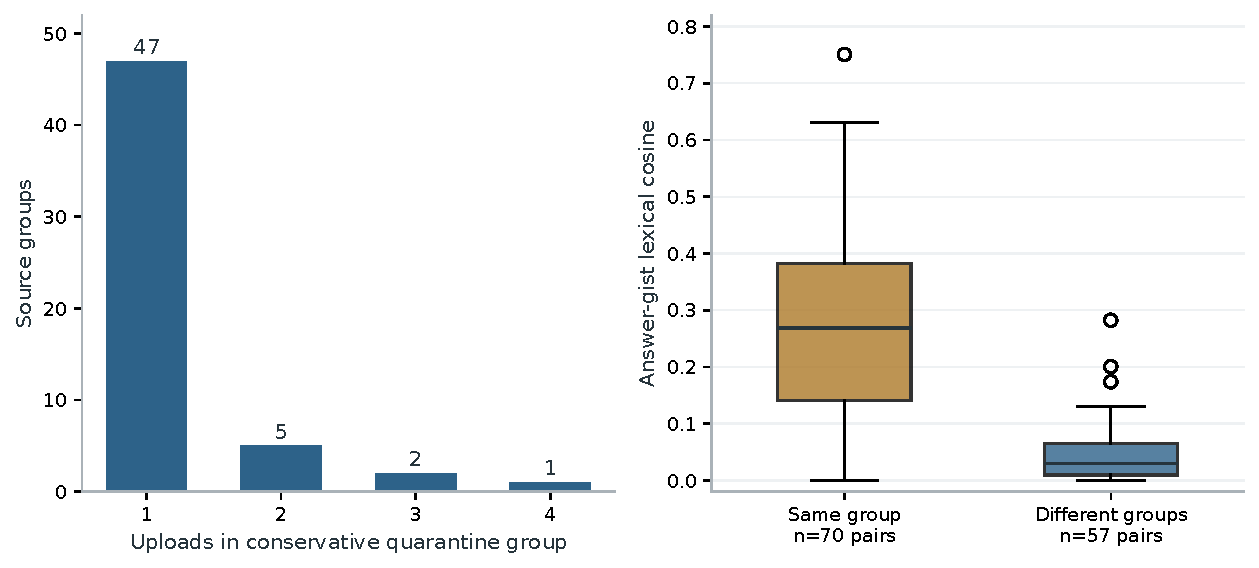
\includegraphics[width=\textwidth]{generated/figures/source-leakage-guard.pdf}
\caption{The conservative source guard changes which question neighbors are compared. Upload links are lexical dependency proxies. Same-group and cross-group pair distributions reuse candidates and are not independent samples or agreement scores.}
\label{fig:source-leakage-guard}
\end{figure*}

\subsection{Question similarity weakly predicts answer wording}

Across 441,797 distinct-upload candidate combinations, question and answer-gist lexical cosines have Spearman rank correlation 0.075. Aggregating to upload-pair means changes the association to 0.323. The change shows sensitivity to weighting and dependence, not a new independent sample.

The 127 question neighbors at cutoff 0.40 have mean answer-gist cosine 0.171. Restricting them to different quarantine groups leaves 57 pairs with mean 0.044. The 15 pairs with identical normalized question wording still have mean answer-gist cosine 0.311. None of these scores codes whether answers agree. Quarantine groups are themselves defined by exact/high question similarity or multiple retrieval links; this selected-pool change cannot isolate a source-reuse effect.

A second, explicitly exploratory comparison standardizes the within- and cross-quarantine answer means over question-cosine bins that contain both strata. The common-support pool contains 93 pairs (36 within and 57 cross), excluding 34 within-group pairs in high-similarity bins with no cross-group support. Pooled-bin weights applied identically to both strata give mean answer cosine 0.297 versus 0.044, a difference of 0.253. The directional within-group advantage is not disconfirmed by this sensitivity, but coarse bins leave prompt, length, topic and source-selection differences unresolved.

\begin{table*}[t]
\centering\small\setlength{\tabcolsep}{3pt}
\begin{tabular}{p{0.2\textwidth}p{0.12\textwidth}p{0.12\textwidth}p{0.17\textwidth}p{0.17\textwidth}p{0.12\textwidth}}
\toprule
Question-cosine band & Within pairs & Cross pairs & Within answer mean & Cross answer mean & Weight \\ \midrule
0.40--<0.50 & 16 & 38 & 0.356 & 0.039 & 0.581 \\
0.50--<0.60 & 14 & 12 & 0.203 & 0.026 & 0.280 \\
0.60--<0.70 & 6 & 7 & 0.243 & 0.104 & 0.140 \\
0.70--<0.80 & 10 & 0 & 0.229 & unavailable & excluded \\
0.80--<0.90 & 6 & 0 & 0.310 & unavailable & excluded \\
0.90--1.00 & 18 & 0 & 0.280 & unavailable & excluded \\
\bottomrule
\end{tabular}
\caption{Question-similarity common support. Standardization uses identical pooled-bin weights only where both quarantine strata occur. Missing cross-stratum means are not zero. These dependent-pair summaries are neither agreement scores nor causal estimates.}
\end{table*}

\begin{figure*}[t]
\centering
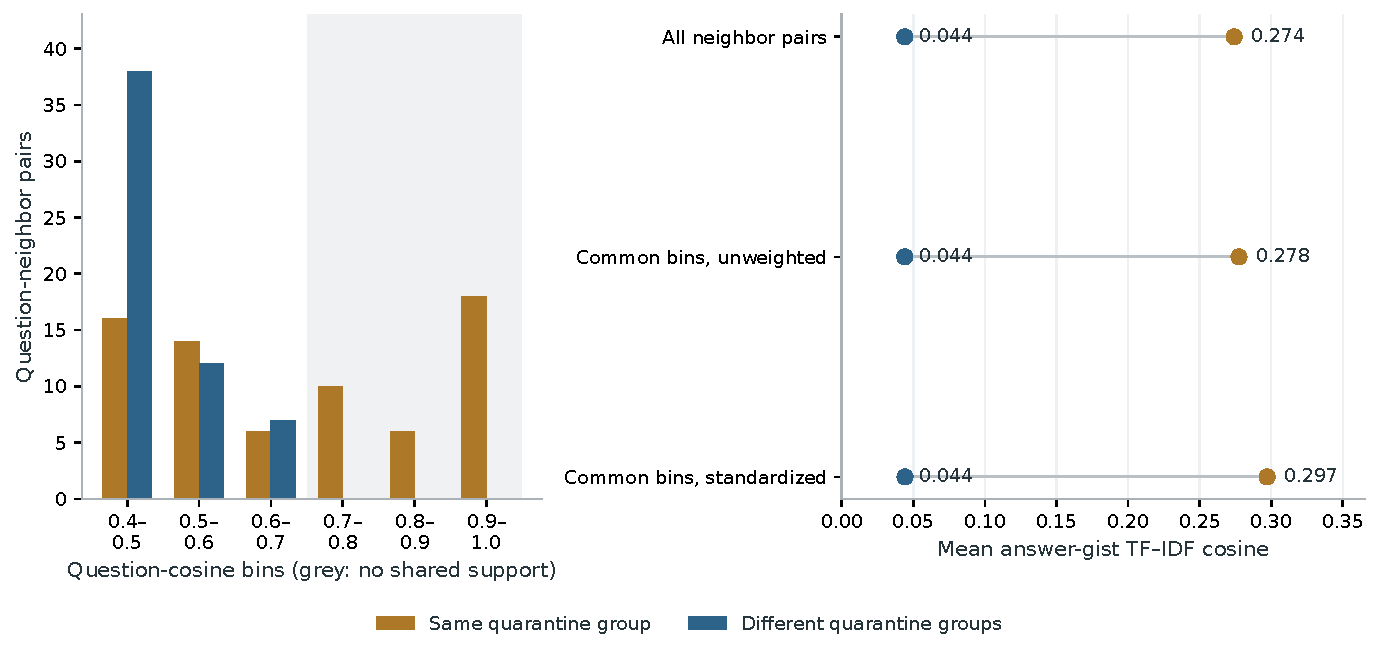
\includegraphics[width=\textwidth]{generated/figures/question-cosine-common-support.pdf}
\caption{Question-similarity support and standardized answer-gist contrast. Only three bins contain both strata: 93 retained pairs and 34 excluded higher-similarity within-group pairs. Identical pooled-bin weights yield descriptive means, with null unsupported comparisons. Group construction and remaining within-bin differences prevent a causal reuse or agreement interpretation.}
\label{fig:question-cosine-common-support}
\end{figure*}

\begin{figure*}[t]
\centering
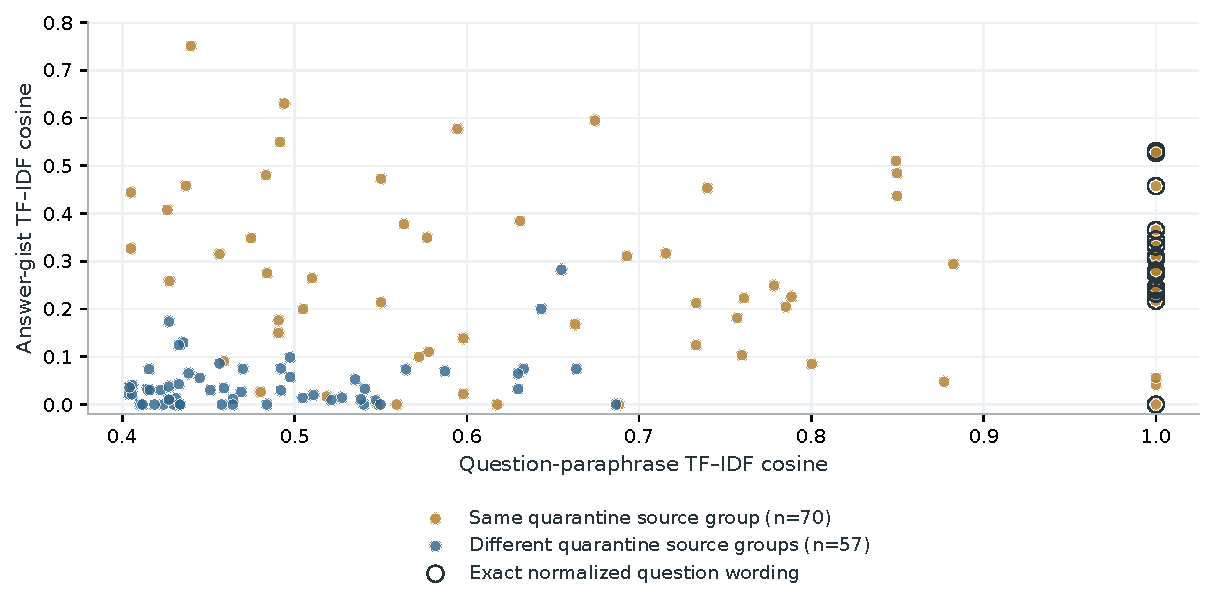
\includegraphics[width=\textwidth]{generated/figures/question-answer-alignment.pdf}
\caption{Question and answer-gist lexical resemblance on source-addressable candidate pairs. Question and answer TF--IDF fits are separate. The quarantine contrast is a dependency sensitivity, not a causal source effect or a semantic agreement validation.}
\label{fig:question-answer-alignment}
\end{figure*}

\subsection{Lexical neighborhoods change with their retrieval threshold}

At question cutoff 0.40, 178 of 949 candidates participate in nonsingleton lexical components; the largest contains 15 candidates. Raising the cutoff to 0.90 leaves 30 linked candidates and a largest component of 3. These are graph neighborhoods under a word-based rule, not validated topic clusters.

\begin{table}[t]
\centering\small\setlength{\tabcolsep}{3pt}
\begin{tabular}{p{0.2\columnwidth}p{0.15\columnwidth}p{0.23\columnwidth}p{0.29\columnwidth}}
\toprule
Cosine cutoff & Edges & Linked Qs & Largest component \\ \midrule
0.40 & 127 & 178 & 15 \\
0.50 & 73 & 114 & 10 \\
0.60 & 47 & 78 & 4 \\
0.70 & 34 & 58 & 3 \\
0.80 & 24 & 39 & 3 \\
0.90 & 18 & 30 & 3 \\
\bottomrule
\end{tabular}
\caption{Lexical graph sensitivity. Isolated candidates remain part of the 949-row denominator; graph connectivity is not original-session identity.}
\end{table}

\begin{figure*}[t]
\centering
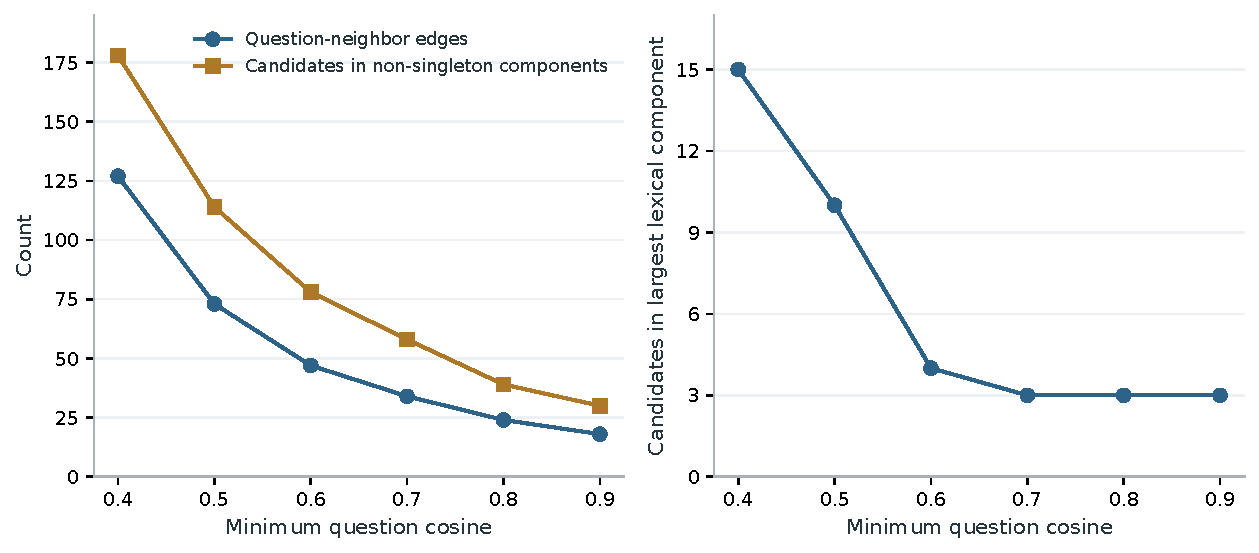
\includegraphics[width=\textwidth]{generated/figures/lexical-graph-stability.pdf}
\caption{Lexical-neighbor connectivity as the question cosine cutoff changes. Vertices are digest candidates and edges link different uploads. Component size reflects the chosen retrieval rule rather than a calibrated semantic or ontological category.}
\label{fig:lexical-graph-stability}
\end{figure*}

\subsection{Text-layer association changes after length conditioning}

The matched representation analysis uses 25 uploads from 14 publishers, yielding 300 dependent upload pairs (11 within publisher, 289 between). Raw title/caption cosine rank association is 0.249. After separate rank projections on absolute log duration ratio, mean log duration and absolute log caption-word ratio, the residual association is 0.129. Publisher omission yields -0.026--0.207, an influence range rather than a confidence interval.

Caption within-minus-between separation changes from 0.154 to 0.133 under the documented conditioning, while title separation changes from 0.229 to 0.217. These descriptive residual comparisons do not identify causal mediation or remove speaker and editing differences.

\begin{figure*}[t]
\centering
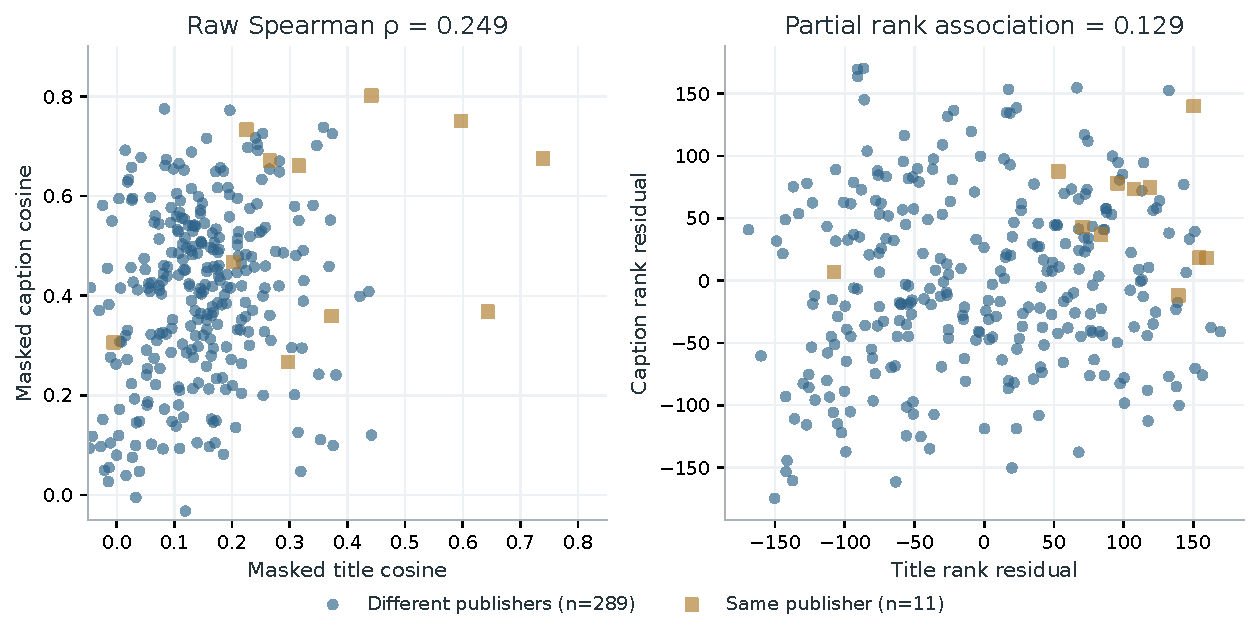
\includegraphics[width=\textwidth]{generated/figures/caption-duration-controls.pdf}
\caption{Title/caption association before and after measured length conditioning on identical uploads. Partial rank association is the correlation of separately projected rank residuals. Pair entries share uploads; publisher-omission ranges measure influence.}
\label{fig:caption-duration-controls}
\end{figure*}

\subsection{Local generation and adaptation pilot}

The executed pilot uses \texttt{Qwen/Qwen2.5-0.5B-Instruct}, revision \texttt{7ae557604adf} (full revision in the run receipt), under its Apache-2.0 license. It uses 48 training examples from 47 source-proxy groups and 8 questions from 8 disjoint groups, plus 2 unsupported-input controls. The retrieval store contains only the training examples; held-out answers are deliberately absent. This is a sparse-source transfer stress test, not a conventional factual RAG benchmark with known answer-bearing documents.

\begin{table*}[t]
\centering\small\setlength{\tabcolsep}{3pt}
\begin{tabular}{p{0.34\textwidth}p{0.15\textwidth}p{0.22\textwidth}p{0.2\textwidth}}
\toprule
Arm & Token F1 & Seconds / response & Strict control marker \\ \midrule
Lexical retrieval & 0.035 & 0.0004 & 1/2 \\
Base closed-book & 0.060 & 1.3962 & 0/2 \\
Base + retrieval & 0.011 & 1.3260 & 1/2 \\
LoRA closed-book & 0.145 & 3.2899 & 0/2 \\
LoRA + retrieval & 0.012 & 1.7715 & 2/2 \\
\bottomrule
\end{tabular}
\caption{Eight held-out question gists and two controls per arm. F1 is lexical overlap with an AI-produced reference gist. Control column counts exact INSUFFICIENT\_EVIDENCE marker emission, not all semantic refusal. The extractive baseline copies a full gist; generators are capped at 40 new tokens. Latency excludes model loading and index fitting. No model-quality ranking is inferred.}
\end{table*}

LoRA executes 48 microsteps and 12 optimizer updates over one epoch in 65.04 seconds, adapting 270,336 of 494,303,104 parameters. Rank is 4 with alpha 8, learning rate 0.0002, gradient accumulation 4, and targets \texttt{q\_proj} and \texttt{v\_proj}. Peak process RSS is 3.21 GiB. This is a short adaptation smoke test on a shared CPU, not an optimized training study or CPU/GPU comparison.

Closed-book reference overlap changes from 0.060 to 0.145 after adaptation, while retrieval-conditioned values are 0.011 and 0.012. The missing held-out answers in the retrieval store confound any algorithm ranking: low overlap may accompany appropriate refusal or evidence gaps. Both language-model retrieval arms emit no valid evidence-label citation on the held-out questions. Citation compliance is therefore an observed failure, separate from source entailment.

The strict control score counts a literal marker. A base response saying ``Insufficient evidence. is a semantic refusal but does not match that marker; zero strict score must not be described as zero refusal. Conversely, the adapted closed-book output supplies a studio temperature of 23 degrees Celsius although no measurement evidence is provided. This concrete unsupported assertion is a substantive failure that token F1 cannot diagnose. The controls are diagnostic examples, not a representative hallucination rate.

A separately disclosed post-hoc phrase diagnostic was defined after inspecting the responses; it does not replace the original metric. It matches refusal expressions such as ``insufficient evidence with spaces/underscores and ``not available. It is another lexical rule, not a human semantic-refusal annotation.

\begin{table}[t]
\centering\small\setlength{\tabcolsep}{3pt}
\begin{tabular}{p{0.43\columnwidth}p{0.24\columnwidth}p{0.24\columnwidth}}
\toprule
Arm & Strict marker & Post-hoc phrase hits \\ \midrule
Lexical retrieval & 1/2 & 1/2 \\
Base closed-book & 0/2 & 2/2 \\
Base + retrieval & 1/2 & 2/2 \\
LoRA closed-book & 0/2 & 1/2 \\
LoRA + retrieval & 2/2 & 2/2 \\
\bottomrule
\end{tabular}
\caption{Control diagnostics on the same two unsupported inputs per arm. The post-hoc phrase rule was selected after viewing outputs and is not an independent validation set.}
\end{table}

Four additional answer-present positive controls supply an exact training-source question and gist, separately for base and adapted retrieval. They are not held-out tests and are excluded from the original five-arm table. Of 4 outputs, 2 exactly reproduce the supplied gist under token-overlap F1, yet 0 emit a valid evidence-label citation. Source availability therefore does not repair citation compliance in this diagnostic. Reproducing an attributed source assertion remains distinct from externally verifying it.

Generation is greedy, float32, limited to 40 new tokens and a 512-token prompt. No prompt was truncated; 5 adapted closed-book and 1 adapted retrieval responses hit the generation cap. Length-limited outputs can lose qualifications and depress lexical overlap. Their full outputs and source evidence remain inspectable in the prediction archive.


\begin{figure*}[t]
\centering
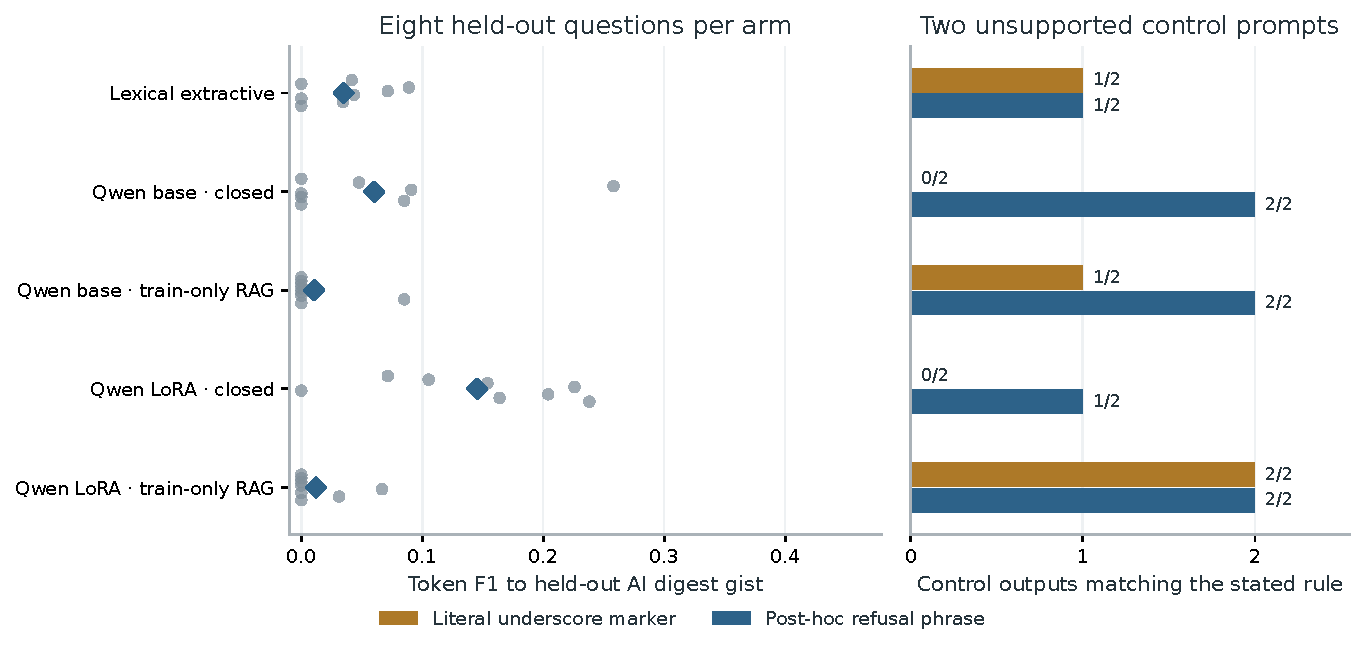
\includegraphics[width=\textwidth]{generated/figures/model-reconstruction-controls.pdf}
\caption{Five executed pilot arms: held-out lexical gist overlap, strict control-marker emission (gold) and the separately defined post-hoc refusal-phrase rule (blue). Eight references are AI digest gists; two controls test unsupported inputs. Neither control rule is human refusal accuracy. Train-only retrieval excludes held-out answers, so these quantities do not rank factual model quality.}
\label{fig:model-reconstruction-controls}
\end{figure*}

\subsection{Structured content labeling exposes another failure mode}

An additional base-model task inspects 12 digest excerpts from distinct source-proxy groups, balanced by a dictionary conditionality marker. It requests a primary answer-orientation label, a conditionality label and an exact evidence span of at most eight words. Only 9 outputs parse under the requested schema; 3 remain recorded failures. Conditional labels match the dictionary method in 5/9 parseable cases. This is method concordance on a selected set, not human annotation accuracy.

The most frequent parsed primary label is contact\_forecast (9/9 parseable outputs). Conditional wording is labeled yes in 9/9 parseable cases, so the reported dictionary concordance is compatible with a collapsed single-label response. Only 0 of 9 parseable evidence spans satisfy the exact-short-span rule. Forced single labels and overlapping dictionary categories are not equivalent tasks. These failures argue for retaining raw outputs and explicit unknown/parse states before using generated labels to characterize this material; they do not establish corpus-wide topic prevalence.

A final same-item probe changes only the listed theme-option order, keeping the twelve excerpts, conditional options and generation settings fixed. Original and reversed prompts each yield 9 parseable outputs, with 8 items parseable in both conditions. Of those paired items, 6 change primary theme. The reversed list yields 7 personal-practice and 2 contact/forecast labels, but selects the new first option in 0/9 parseable outputs. This disconfirms a simple first-option-copying explanation while demonstrating local prompt-order sensitivity. No reversed output satisfies the combined exact-short-span rule.

A separate post-hoc dictionary sensitivity narrows the broad dependency-word expression. Conditional flags change from 60 to 58 among 949 source gists (2 changed records). Neither rule is a human reference, and the original selection and benchmark labels remain unchanged. Stability under this single lexical perturbation does not validate the conditionality construct.

The newer pinned Qwen3.5-0.8B model then executes the same twelve excerpts and original annotation schema/options with a 96-token cap, greedy decoding and thinking disabled. It returns 12/12 parseable outputs and 5/12 exact answer substrings of at most eight words, compared with 9/12 and 0/9 in the original small-model run. Its conditional labels are yes in 12/12 cases: 6/12 dictionary concordance is exactly the always-yes result on the balanced six/six sample. Primary labels remain concentrated (11 personal-practice, 1 contact/forecast).

Thus parsing and short-span compliance improve in this same-item check while conditional-label collapse persists. Of the newer model's 12 evidence strings, 10 are exact contiguous answer substrings; 5 of those exceed eight words, leaving 5 combined exact-short successes and 2 nonexact strings. Exact but overlength spans are length-compliance failures, not invented evidence. The modern model uses its own tokenizer/chat template and runtime; architecture, instruction behavior and those implementation changes are not isolated. Mean runtime is 6.90 seconds per excerpt, with 0 cap hits and peak process RSS 5.35 GiB. No human label accuracy, source-truth validation or general model ranking is established.

\begin{table*}[t]
\centering\small\setlength{\tabcolsep}{3pt}
\begin{tabular}{p{0.25\textwidth}p{0.16\textwidth}p{0.18\textwidth}p{0.18\textwidth}p{0.16\textwidth}}
\toprule
Annotation condition & Parsed / selected & Exact spans / parsed & Exact + short / parsed & Primary labels \\ \midrule
Qwen2.5 original & 9/12 & 0/9 & 0/9 & 9 contact/forecast \\
Qwen2.5 reversed options & 9/12 & 0/9 & 0/9 & 7 personal practice; 2 contact/forecast \\
Qwen3.5 original options & 12/12 & 10/12 & 5/12 & 11 personal practice; 1 contact/forecast \\
\bottomrule
\end{tabular}
\caption{Same selected excerpts, explicitly different prompt/model conditions. Exact means a nonempty contiguous answer substring; the combined criterion also requires at most eight whitespace words. Source labels are model outputs, not measured corpus prevalence or human annotation accuracy.}
\end{table*}

\subsection{Newer-family execution is a separate compatibility probe}

A separately pinned \texttt{Qwen/Qwen3.5-0.8B} model, revision \texttt{2fc06364715b}, also executes on CPU using \texttt{Transformers 5.20.2}. The single text-only prompt directly supplies the desired provenance values (AI digest and unverified speaker turns) and requests a JSON object. The response follows that schema. This is instruction-following compatibility, not independently inferred provenance, domain accuracy or a comparison with the earlier labeling task.

The probe generates 23 tokens under a 32-token limit in 3.88 seconds after 1.03 seconds of model loading, with peak process RSS 5.33 GiB. The architecture supports image/text inputs, but no image, video, audio or speech-recognition input is used. Its different prompt and budget make it separate from the five-arm Qwen2.5 experiment; no state-of-the-art, model-quality or CPU/GPU ranking follows.


\section{Discussion}
\subsection{The answer depends on the evidentiary unit}
The linked pipeline makes several useful research actions possible before a multi-practitioner answer study is available: retrieve source-addressable questions, inspect associated gists, identify possible reuse, audit publisher composition and compare model outputs against their accessible evidence. These capabilities address a practical source-understanding problem. They do not justify converting multiple publishers into multiple independent practitioners.

Questions about life direction, beliefs, contact or consciousness can recur within one practitioner context. Repetition may reflect audience concerns, a stable teaching vocabulary, source reuse or summary normalization. The separate question, answer and source fields allow these explanations to compete. A high-dimensional vector alone cannot choose among them. When a retrieved pair disagrees with a model-assisted reading, it becomes an inspection target rather than an error to remove by selecting a preferred encoder.

\subsection{Retrieval and adaptation solve different operational problems}
A closed-book model responds from its pretrained parameters and prompt. Retrieval supplies identifiable context. Adaptation changes response behavior using the training examples. Differences among these arms can therefore arise from evidence access, response length, formatting or memorization, in addition to any useful improvement in source handling. A model that copies a reference phrase can obtain higher token F1 without preserving its qualifications. A source-linked response can remain unsupported even when its cited identifier exists.

The correct interpretation of a small CPU pilot is consequently operational and bounded. It can establish that a chosen runtime, model artifact, split and training configuration execute, and expose concrete output failure modes. A larger validation study would compare equal evidence budgets, assess groundedness and relevance with held-out human judgments, and retain negative results. It should also test whether improvements survive source-family exclusion and prompt paraphrase.

\subsection{Novelty and substantive scope}
Channeling content analysis, account embeddings, lexical retrieval, RAG and low-rank adaptation all have prior work. Our proposed contribution is their source-typed integration in a traceable research resource, plus the concrete measurement and failure analyses that integration enables. The work is not a new embedding algorithm, a validated truth detector or a first-in-field claim derived from incomplete search.

The substantive object is how attributed communications are published, summarized and computationally represented. Similarity, repeated answers or generated fluency do not determine extraterrestrial origin, independent information or clinical state. This boundary leaves meaningful social-computing questions: who publishes which formats, how titles differ from speech, which questions recur, how reuse affects comparison, and when systems preserve or erase source uncertainty.

\section{Limitations and Responsibility}
The index is purposive, English-biased and historically mixed, with unknown inclusion probabilities. Empty or unresolved account routes, unavailable captions and approximate identity joins remain. Known-ID refresh and keyword enumeration cannot establish a worldwide active-medium count. Upload dates do not necessarily date performances or current activity.

The derivative Q\&A corpus concerns one practitioner context and may inherit summarizer omissions or normalized wording. It has no new human-verified answer speakers or literal turn timestamps. Captions are largely automatic and unsegmented; model-assisted readings do not establish caption accuracy, human agreement or participant interpretation. Source-family graphs are conservative proxies rather than verified performance identities.

The model pilot is small, CPU-constrained and tied to one baseline and one derivative corpus. Token F1, citation syntax and simple abstention rules are partial measurements. Test rows can still share latent teachings, summarization style or pretraining exposure with training material despite the grouping guard. Small controls and model-agent readings do not replace held-out human evaluation.

Public professional records are analyzed without private communications or audience profiling. Raw captions, full third-party transcript bodies, credentials and model weights are excluded from public research artifacts unless an explicit release basis is established. Model outputs can contain unsupported claims and are displayed as generated research outputs. Appropriate institutional determination, rights review, human authorship, affiliations and contributor acceptance remain \textbf{TBD}. The living draft is not submitted or accepted. The official ICWSM/AAAI preprint style is used as a writing reference; venue compliance must be assessed for a concrete submission.

\section{Conclusion}
Source-grounded computational research begins by preserving what each record actually is. This continuation links a heterogeneous video index to typed Q\&A candidates, source-dependency diagnostics and a bounded local modeling workflow. The resulting analyses make publishing structure, lexical reuse and evidence access inspectable, while the paper and dashboard share reproducible inputs. The next substantive step is attributable multi-practitioner answer material with human-reviewed prompts, speakers and claims. More computation can help organize that evidence, but it does not substitute for obtaining and validating it.

\section*{AI and Review Disclosure}
Model-agent workstreams assisted acquisition, literature inspection, database and model experiments, quantitative analysis, interface implementation and manuscript development. Three new continuation loops, numbered 10--12, review implemented artifacts and record corrections separately from prior rounds. Their receipts name actual files and hashes; they are not independent human peer review. Human responsibility for final authorship and acceptance remains pending.
